\documentclass{article}

\usepackage[utf8]{inputenc}
\usepackage[T1]{fontenc}
\usepackage{lipsum}
\usepackage{graphicx}
\usepackage{amsmath}
\usepackage[margin=1in]{geometry}
\usepackage{titlesec}
\usepackage{enumitem}

\titleformat{\section}
{\LARGE\bfseries}{\thesection}{1em}{}

\titleformat{\subsection}
{\Large\bfseries}{\thesection}{1em}{}

\begin{document}
\pagestyle{empty}
\section*{Design pattern 2}
\large

\subsection*{Introduzione}
\large
Obiettivi:
\begin{itemize}
    \renewcommand{\labelitemi}{-}
    \itemsep0em
    \item Applicare propriamente i pattern del modello GoF 
\end{itemize}
Questa sezione rappresenta il naturale conseguimento del documento \textit{Design Pattern 1}, in cui sono elencati ulteriori pattern \textit{comportamentali}, \textit{creazionali} e \textit{strutturali} del \textit{catologo GoF}.

\subsection*{State (Behavioral Pattern)}
\large
\textit{Problema}\\
Come intercambiare il comportamento di un oggetto dipendente da uno stato tramite una soluzione di alta qualità?\vspace*{14pt}\\
\textit{Soluzione}\\
Definire un meccanismo che permetta ad un oggetto di variare il proprio comportamento quando lo stato interno dell'oggetto varia.\vspace*{14pt}\\
Il pattern \textbf{State} è una soluzione applicata alla necessità di creare un insieme di comportamenti caratteristici strettamente correlati ad uno stato, che possa acquisire l'oggetto della classe in questione. In relazione all'adozione di un meccanismo di composizione simile, sono adottati sei passi principali:
\begin{itemize}[label={-}]
    \itemsep0em
    \item Creare un layer astratto, quale un'interfaccia, che definisca l'intero contesto a cui una classe possa richiedere di variare il proprio comportamento
    \item Creare una classe astratta da cui deriveranno le classi concrete, ossia che implementano i \textit{behavior} specifici
    \item Rappresentare i differenti stati acquisibili dal sistema software modellato come sottoclassi derivanti dalla classe astratta principale
    \item Implementare il meccanismo comportamentale specifico per ogni singola sottoclasse derivata
    \item Mantenere un riferimento all'interno dell'interfaccia affinchè sia possibile variare il comportamento in base allo stato corrente dell'istanza
    \item Concludendo, per variare lo stato del sistema software, modificando il comportamento associato, semplicemente verrà cambiato il riferimento dello \textit{stato corrente} 
\end{itemize}\vspace*{7pt}
\textit{Caso di studio}\\
Affinchè sia possibile comprendere quando e come applicare al meglio il pattern \textit{State}, di seguito è proposto un esempio grafico che possa raffigurare al meglio quanto detto.\vspace*{7pt}
\begin{center}
    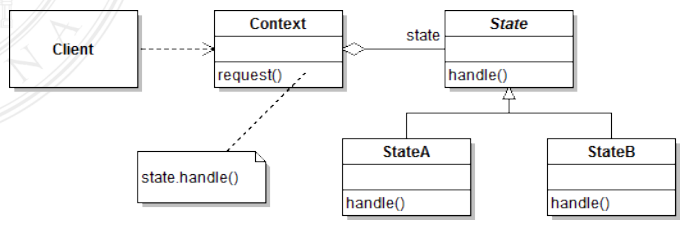
\includegraphics[width=0.7\textwidth]{foto 1.png}
\end{center}
Come da raffigurazione si notano i passaggi elencati precedentemente, in cui la classe \textit{Context} rappresenta il livello di astrazione necessario affinchè sia possibile intercambiare comportamenti di oggetti durante il run time.\\
\textit{Context} a sua volta delega alla classe astratta \textit{State} la responsabilità di implementare il comportamento specifico, in cui in questo caso avviene per uno dei due \textit{behavior} esternalizzati, \textit{StateA} e \textit{StateB}; è bene sottolineare la sottile differenza che vige dal pattern \textit{Strategy}, dove nel meccanismo di delega introdotto la scelta del \textit{behavior} è imposta dall'utente finale, si ricorda il processo modellato, in cui è definita l'architettura generale dell'algoritmo affinchè siano classi derivate a specificarne l'implementazione di step specifici, mentre mediante \textit{State} sarà l'interfaccia ad imporre quale metodo debba essere considerato affinchè sia garantito il cambiamento dello stato corrente, il quale gioca un ruolo fondamentale poichè permette  intercambiabilità del processo comportamentale dell'istanza in questione.\vspace*{14pt}\\
Infine si considera la casistica in cui debbano essere introdotte nuove funzionalità. Dato che si considera lo stretto legame posto tra \textit{comportamento-stato}, ogni volta che si debba implementare un nuovo \textit{behavior} sarà creata una nuova classe derivata che specificherà la logica logaritmica del metodo, ovviando a \textit{design smells}, come \textit{needless repetition}, e violazioni dei principi \textit{SOLID}. 

\subsection*{Factory}
\large
Linguaggi legati al paradigma degli oggetti promuovono l'utilizzo di istanze di classi software, affinchè mediante funzionalità incapsulate al loro interno e una corretta manipolazione delle dipendenze, possano dare vita alla soluzione che soddisfi i requisiti funzionali degli utenti finali.\vspace*{14pt}\\
Tuttavia nella stesura del codice spesso non si pone abbastanza importanza sulla creazione di oggetti, ottenuti tramite la semantica \textit{new (...)}, in cui modifiche all'interno del costruttore di classi concrete potrebbero provocare la rottura dell'operatività di \textit{low level classes}. Una prima soluzione potrebbe consistere nel porre il corretto livello di astrazione tra elementi del modello legati alla \textit{business logic} rispetto a classi adoperate da \textit{UI}.\vspace*{14pt}\\
Nonostante la risoluzione, la quale potrebbe risultare conforme rispetto ai principi del modello \textit{SOLID}, è affetta da un'errata gestione delle dipendenze ed espone \textit{LLC} alla determinazione di classi concrete. Affinchè il tema trattato risulti comprensibile, si visualizza di seguito un caso di studio.\vspace*{14pt}\\
\textit{Caso di studio}\\
Si pensi alla creazione di un sistema software che debba gestire le singole operazioni di un servizio \textit{InBank}, in cui si vuole relegare una qualsiasi transazione di denaro ad una condizione di estrema persistenza. Per cui ponendo due attori \textit{A} e \textit{B}, i quali si scambiano una certa somma di denaro mediante un bonifico bancario, occorre un oggetto che gestisca la transazione di denaro e un'ulteriore istanza che provveda al controllo di persistenza. 
\begin{itemize}[label={ }, leftmargin=1cm]
    \itemsep0em
    \item \textit{FilePersistMgr fpm = new FilePersistMgr();}
    \item \textit{fpm.makePersistent(b)};
\end{itemize} 
Mediante l'ausilio di un file, avviene la scrittura della transazione eseguita dei due conti, dove, tralasciando l'erronea gestione di concorrenza, una soluzione simile non può essere considerata certamente corretta, dato che si prediligie un collegamento diretto tra \textit{low level class}, colei che richiama l'istanza, e \textit{high level class}, ossia la logica logaritmica che permette la scrittura del dato bonifico sul documento. Dato che una \textit{dipendenza} è potenzialmente un percorso che possa diffondere una serie di cambiamenti, si tenta di predire il vincolo comportamentale minimizzando il possibile evento catastrofico che si potrebbe verificare all'interno della soluzione software.\vspace*{14pt}\\
Si passa quindi all'uso di layer astratti, come interfacce, capaci di porre una \textit{schermatura} che consenta ad alcune funzionalità di riportare modifiche solamente ad una delle due parti in gioco, \textit{HLC} oppure \textit{LLC}, ovviando alla possibilità che si possa riverbare sull'intera struttura del sistema software adeguato.
\begin{itemize}[label={ }, leftmargin=1cm]
    \itemsep0em
    \item \textit{PersistMgr fpm = new FilePersistMgr();}
    \item \textit{fpm.makePersistent(b)};
\end{itemize}
In questa maniera è possibile porre l'interfaccia \textit{PersistMgr} come l'artefice della creazione dell'istanza della classe concreta, nonostante questo non garantisca il livello di correttezza voluto.\vspace*{14pt}\\
Giunto a questo punto, interviene la \textit{pure fabrication}, ossia l'idioma \textit{Factory}, in cui il caso di studio diviene:
\begin{itemize}[label={ }, leftmargin=1cm]
    \itemsep0em
    \item \textit{PersistMgr fpm = Factory.createPersistMgr();}
    \item \textit{fpm.makePersistent(b)};
\end{itemize}
Per cui si tende a spostare le responsabilità in ulteriori classi, in cui sarà l'interfaccia \textit{Factory}, in maniera totalmente autonoma, l'artefice della creazione dell'istanza della classe concreta, in cui elementi di basso livello saranno totalmente disinteressati rispetto al processo esecutivo che porti alla realizzazione dell'oggetto desiderato, ponendo quindi il corretto layer di astrazione. 

\subsection*{Factory Method (Creational Pattern)}
\large
\textit{Problema}\\
Come creare un'istanza di una classe senza che sia specificata l'esatta classe?\vspace*{14pt}\\
\textit{Soluzione}\\
Definire un'interfaccia per la creazione di oggetti, la quale permetta alle singole sottoclassi di decidere quale entità debbe essere stanziata.\vspace*{14pt}\\
\textit{Caso di studio}\\
E' bene sottolineare che l'idioma e il pattern della GoF non rappresentino la stessa cosa. In quanto \textit{Factory Method} non indica una classe esterna, come era stato stabilito nel caso di studio precedente, ma raffigura entità relegate a singoli oggetti oppure a certe funzionalità.\vspace*{7pt}
\begin{center}
    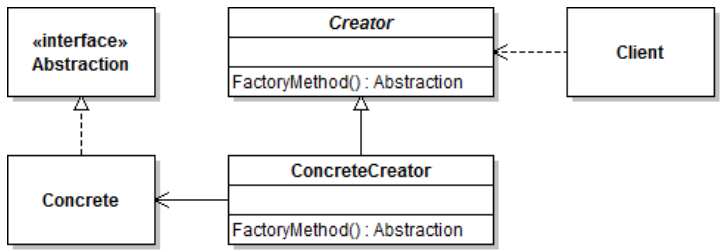
\includegraphics[width=0.6\textwidth]{foto 2.png}
\end{center}
Nel contesto raffigurato è solamente il metodo \textit{FactoryMethod()} che si occupa della creazione della classe concreta. Concettualmente è molto simile al pattern \textit{Template Method}, in cui viene implementata la struttura portante dell'algoritmo, tralasciando a sottoclassi la resposanbilità di implementare certi passaggi come preferiscono. Concludendo, in questo modo il metodo illustrato è legato alla logica algoritmica ed è l'unico di carattere astratto, ovviando alla specifica esatta della classe che voglia essere stanziata.  

\subsection*{Notification}
\large
Il problema relativo alla \textit{notification} può essere espresso come un'avversità pragmatica e contraria alla realizzazione della soluzione. Applicando una semplificazione, spesso questa problematica, piuttosto ricorrente, ritrae componenti soggette a notifiche qualora vari lo stato di elementi correlati. Tuttavia l'intento promuove l'uso di strumenti affinchè l'oggetto notificante non sia dipendente da terze parti. \textbf{Chiedere se ci sta mettere la foto oppure esempio da fare generale ...}\vspace*{14pt}\\
Riassumendo occorre realizzare una soluzione che mantenga in considerazione alcuni principi ritenuti fondamentali, come:
\begin{itemize}[label={-}]
    \itemsep0em
    \item \textit{Protected Variations}, mettere in pratica la descrizione del principio affinchè cambiamenti conseguiti non varino funzionalità già esistenti
    \item \textit{Interface Segregation}, definire un'interfaccia più ridotta possibile che possa contenere la dipendenza dell'oggetto notificante rispetto alla classe in ricezione
    \item \textit{Dipendency Inversion}, dipendere da astrazioni, ossia applicare \textit{abstract layer}, affinchè sia posta una schermatura tra \textit{low level classes} e \textit{high level classes}
\end{itemize}
L'insieme di queste tematiche è affrontato dal \textit{Observe pattern}, il quale ammette:\vspace*{7pt}\\
\textit{Soluzione}\\
Tramite il \textit{pattern} avviene la costruzione di una classe astratta posta tra l'istanza notificante e l'oggetto in ascolto, affinchè tutte le dipendenze della prima citata possano essere automaticamente segnalate oppure aggiornate sul cambiamento di stato.\vspace*{14pt}\\
\textit{Caso di studio}\\
\begin{center}
    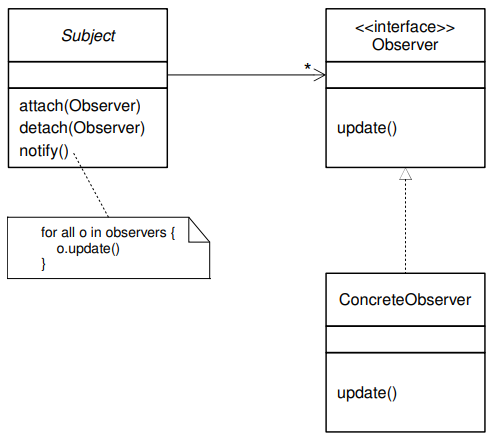
\includegraphics[width=0.4\textwidth]{foto 3.png}
\end{center}
Come da raffigurazione, la classe \textit{Subject} rappresenta l'entità che deve comunicare alle proprie dipendenze il cambiamento del proprio stato, mentre \textit{ConcreteObserver} indica la classe concreta in ascolto o in ricezione di modifiche, ossia il vincolo comportamentale prima definito. Ribadito più volte in altri contesti simili, l'uso di un'interfaccia astratta permette di interrompere lo stretto collegamento tra le classi in questione, eliminando ogni stretta correlazione, rispettando soprattutto i tre principi prima elencati.\vspace*{7pt}\\
Piccola nota è relativa ai metodi implementati da \textit{Subject}, in cui \textit{attach()} è implementato per aggiungere un osservatore, \textit{detach()} permette di eliminare una dipendenza dell'elenco di notifica infine \textit{notify()} garantisce l'aggiornamento a tutti gli osservatori. 
\end{document}